% Boolean indexing on the first five students (values checked in kmeans_start.py):
% X, the labels y_means, the mask y_means == 1, and what X[y_means == 1, 0] keeps.
\documentclass[tikz,border=8pt]{standalone}
% Shared look for every TikZ diagram. Load with \input{../../tools/tikz-style.tex}
\usepackage[T1]{fontenc}
\usepackage{lmodern}
\renewcommand{\sfdefault}{lmr}  % diagrams use the same serif as the text
\usetikzlibrary{arrows.meta, positioning, shapes.geometric, calc, fit, backgrounds}
\definecolor{cblue}{HTML}{4C78A8}
\definecolor{corange}{HTML}{F58518}
\definecolor{cgreen}{HTML}{54A24B}
\definecolor{cred}{HTML}{E45756}
\definecolor{cpurple}{HTML}{B279A2}
\definecolor{cgrey}{HTML}{6B6B6B}
\tikzset{
  every picture/.style={font=\sffamily, line width=1.2pt},
  box/.style={draw=#1, fill=#1!12, rounded corners=4pt, align=center, inner sep=7pt, minimum height=1.1cm},
  box/.default=cgrey,
  arrow/.style={-{Stealth[length=3mm]}, draw=cgrey, line width=1.4pt},
  title/.style={font=\sffamily\bfseries\Large},
  note/.style={font=\sffamily\small, text=cgrey, align=center},
}
\AtBeginDocument{\hyphenpenalty=10000 \exhyphenpenalty=10000}

\usepackage{ifthen}
\begin{document}
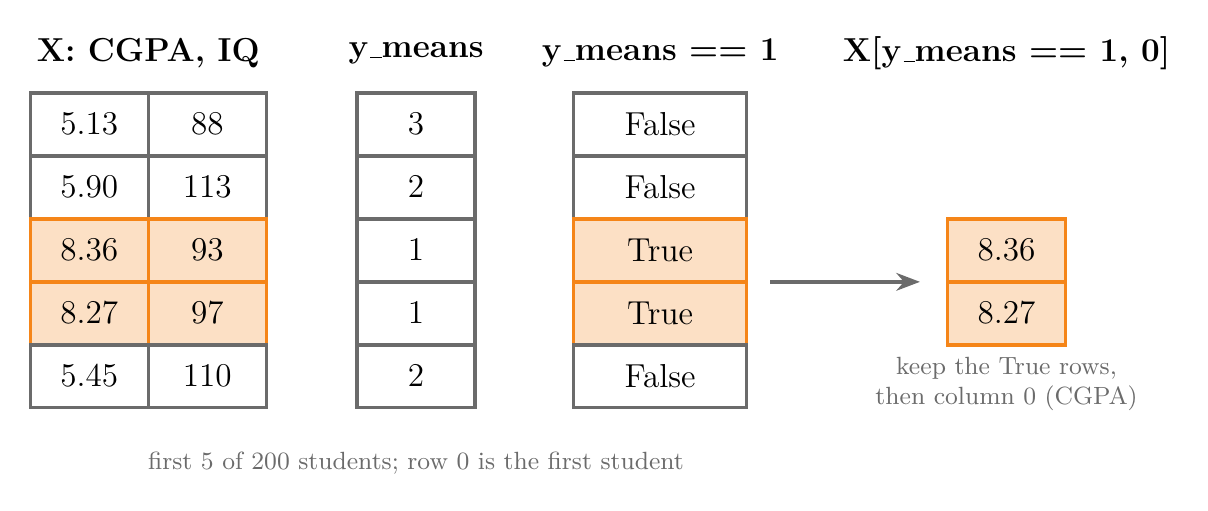
\begin{tikzpicture}[cell/.style={draw=cgrey, minimum width=1.5cm, minimum height=0.8cm, font=\sffamily\large},
  hit/.style={cell, fill=corange!25, draw=corange}, head/.style={font=\sffamily\bfseries\large, align=center}]
  \node[head] at (1.5,0.9) {X: CGPA, IQ};
  \node[head] at (4.9,0.9) {y\_means};
  \node[head] at (8.0,0.9) {y\_means == 1};
  \node[head] at (12.4,0.9) {X[y\_means == 1, 0]};
  \foreach \i/\c/\q/\l/\m in {0/5.13/88/3/False, 1/5.90/113/2/False, 2/8.36/93/1/True, 3/8.27/97/1/True, 4/5.45/110/2/False} {
    \pgfmathsetmacro{\y}{-0.8*\i}
    \ifthenelse{\equal{\m}{True}}{\def\s{hit}}{\def\s{cell}}
    \node[\s] at (0.75,\y) {\c}; \node[\s] at (2.25,\y) {\q};
    \node[cell] at (4.9,\y) {\l};
    \node[\s, minimum width=2.2cm] at (8.0,\y) {\m};
  }
  \node[hit] (a) at (12.4,-1.6) {8.36};
  \node[hit] (b) at (12.4,-2.4) {8.27};
  \draw[arrow] (9.4,-2.0) -- (11.3,-2.0);
  \node[note] at (4.9,-4.3) {first 5 of 200 students; row 0 is the first student};
  \node[note] at (12.4,-3.3) {keep the True rows,\\then column 0 (CGPA)};
\end{tikzpicture}
\end{document}
